\section{Theory}
\subsection{Droplet motion}
The basis of this investigation lies on the motion of moving droplets on a liquid surface. In 1978 it was reported by J. Walker \cite{Walker} that droplets vibrating at a certain frequency upon a soap-solution surface would not immediately coalesce, but could maintain motion for up to 18 minutes. Couder \textit{et al.} further researched this phenomenon in 2005. Using a silicon oil surface(with no soap-substrate) they discovered that it was possible to create a   an oscillating droplet at certain frequencies, and even walking droplets that moved parallel to the surface. 
The walking droplets were created by simply vibrating the liquid surface vertically at a frequency determined by Equation \ref{eq:bouncing regime condition}:

\begin{equation} \label{eq:bouncing regime condition}
\frac{\gamma_{m}^{B}}{g}\approx 1
\end{equation}
Where $g$ is the acceleration due to gravity, $\gamma_{m}^{B}$ is the specific value of co-efficient $\gamma_{m}$ of Equation \ref{eq:vertical acceleration}: 


\begin{equation} \label{eq:vertical acceleration}
\gamma=\gamma_{m}cos(2 \pi f_0t) 
\end{equation}

Equation \ref{eq:vertical acceleration} determines $\gamma$, which is the vertical acceleration of the fluid, $f_0$ is the driving frequency of the liquid and $t$ is time. The droplets bounce due to a remarkably simple mechanism. Upon collision of a droplet with the liquid, there exists a thin layer of air trapped between the two surfaces. Normally, the droplet will coalesce with a surface in a matter of seconds, as this air is forced away. But above a threshold value of $\gamma_{m}$, the droplet will instead bounce, as the air film retains its integrity, forcing the droplet upwards. By specifying a threshold vertical acceleration, it is also ensured that the air film will have a chance to replenish after each subsequent bounce, allowing the motion to be periodic over a large period of time. The regimes in which different types of motion occur are described in Figure \ref{regimes}

\begin{figure}[ht]
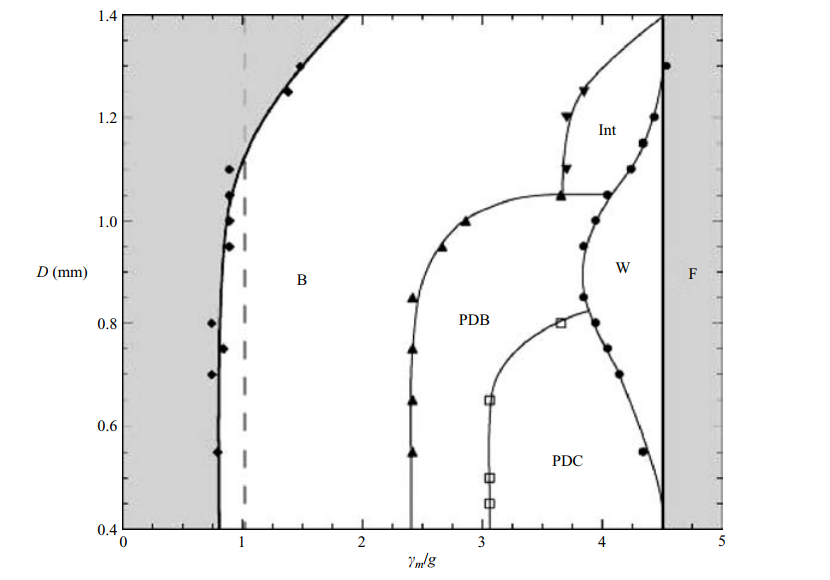
\includegraphics[width=12cm]{theory/regime}
\centering
\caption{A graph of droplet Diameter against $\frac{\gamma_{m}}{g}$ for an oscillating droplet in a vibrating liquid. It illustrates the different vertical acceleration regimes: Bouncing(B), Walking(W), Faraday instability(F), Period Doubling (PDB), transition from Periodic to chaotic behaviour(PDC)  and Intermittent behaviour(Int).}
\centering
\label{regimes}
\end{figure}

Furthermore, droplets can also exhibit motion parallel to the droplet surface. Such droplets are labelled walkers, and like bouncing droplets, they exist in a certain $\frac{\gamma_{m}}{g}$ regime, just below the onset of the Faraday instability. The Faraday instability can be defined as the point at which a surface becomes spontaneously wavy. Just before its onset, a bouncing droplet has a period of motion twice that of its driving oscillation. It thus generates a damped travelling Faraday wave at each bounce where Faraday waves are standing waves generated by a vibrating liquid. The subsequent landing then occurs on the reverse slope of this previously generated Faraday wave. This landing generates another travelling Faraday wave, and causes the droplet to perform a parabolic bounce, causing motion parallel to the surface. An intuitive way to understand this motion is to imagine jumping on a trampoline. Each time you land on the trampoline, a wave is generated. If you land again anywhere but at the centre of this wave, you spring off again, and your motion has a slight horizontal component, allowing you to travel around the trampoline. As the wave you generate when landing travels, you constantly land on its side, therefore there is a constant horizontal motion, allowing you to 'walk' around the trampoline. This motion is illustrated in Figure \ref{walker}: 

\begin{figure}[htbp]
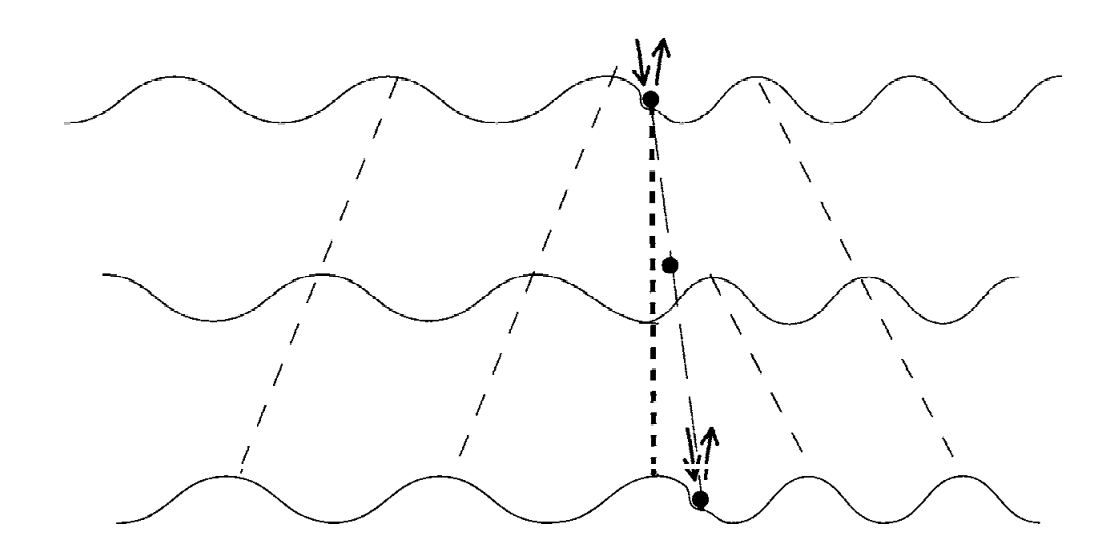
\includegraphics[width=12cm]{theory/walkingDroplet}
\centering
\caption{An illustration of a walking droplet's motion for subsequent bounces. The movement of droplet is exaggerated for visual purposes. In reality, wave amplitude decays with distance from droplet and is not necessarily constant; it is modulated by the driving force }
\centering
\label{walker}

\end{figure}

\subsection{Pilot Wave Theory}
Pilot Wave Theory, also known as the De Broglie-��Bohm theory, is an alternative deterministic interpretation to quantum mechanics. 

It proposes that a 'hidden equation' is partly responsible for determining the measurements of a system, and that this measurement result exists prior to measurement. For a single particle case, this guiding equation is specified as Equation \ref{eq:pilot wave}: 

\begin{equation} \label{eq:pilot wave}
\frac{d\mathbf{Q}}{dt}(t) = \frac{\hbar}{m} \mathrm{Im}\left(\frac{\nabla \psi}{\psi}\right)(\mathbf{Q}, t)
\end{equation}


Where $Q$ is the 'configuration space', $\psi$ is the particle wave-function, $m$ is the particle mass and $\hbar$ is the reduced Planck constant. 

This is unlike the Copenhagen interpretation where, as an example, the velocity of a particle is only known after measurement. Pilot Wave Theory also satisfies nonlocality, or the idea that a system of particles separated by a large distance can instantaneously know of each others state. As the pilot wave equation and Schrodinger's equation jointly specify the velocity of a particle according to the position of other particles in the defined 'universe', there is a necessary inter-dependency that is not local to the particle's position. 

Surprisingly enough, on a macroscopic level, Pilot Wave Theory is very well described by the motion of droplets on a vibrating surface, and the subsequent Faraday waves. In the following discussion, quantum mechanical effects and their analogies to this droplet system will be introduced:

\subsection{Section about discussion of Me parameter and it's influence on walking states}

\subsection{May need section on interaction between multiple droplets if we use that data}

\subsection{Fluid Dynamics}
If the height of the oil is known for the entire surface of the oil, 